\documentclass[12pt]{article}

\usepackage[utf8]{inputenc}
\usepackage{setspace}
\usepackage{geometry}
\usepackage{graphicx}
\usepackage{caption}
\usepackage{indentfirst}
\usepackage{anyfontsize}
\usepackage{textcomp}
\usepackage{float}

\graphicspath{}



\title{SIR Influenza Modeling}
\author{Geneva Porter}
\date{25 September 2018}

%\begin{figure}[H]
%\centering{\includegraphics[width=10cm]{FILENAME.eps}}
%	\caption*{Figure xxx}
%\end{figure}

\begin{document}
	
\begin{titlepage}
\maketitle
\thispagestyle{empty}



\centering
\large \it San Diego State University

Professor Mahaffy, Math 636
\end{titlepage}

\section*{SIR Model with Preventative Measure Comparison}

SIR is the Susceptible $\rightarrow$ Infected $\rightarrow$ Recovered shorthand when discussing disease spread and control. Infectious disease is a complex and important issue with global repercussions. Here we examine an influenza outbreak in a population of $\approx$ 150,000 over 48 weeks. Figure 1 shows the data collected on cases of the flu as well as a best-fit model with optimized $\beta$ and $\gamma$ parameters. This model fits the data fairly accurately, yet underestimates the peak infected point. There also appears to be a sharp increase in infected individuals around week 12, which may be due to a large, indoor gathering. 




\begin{figure}[H]
\centering{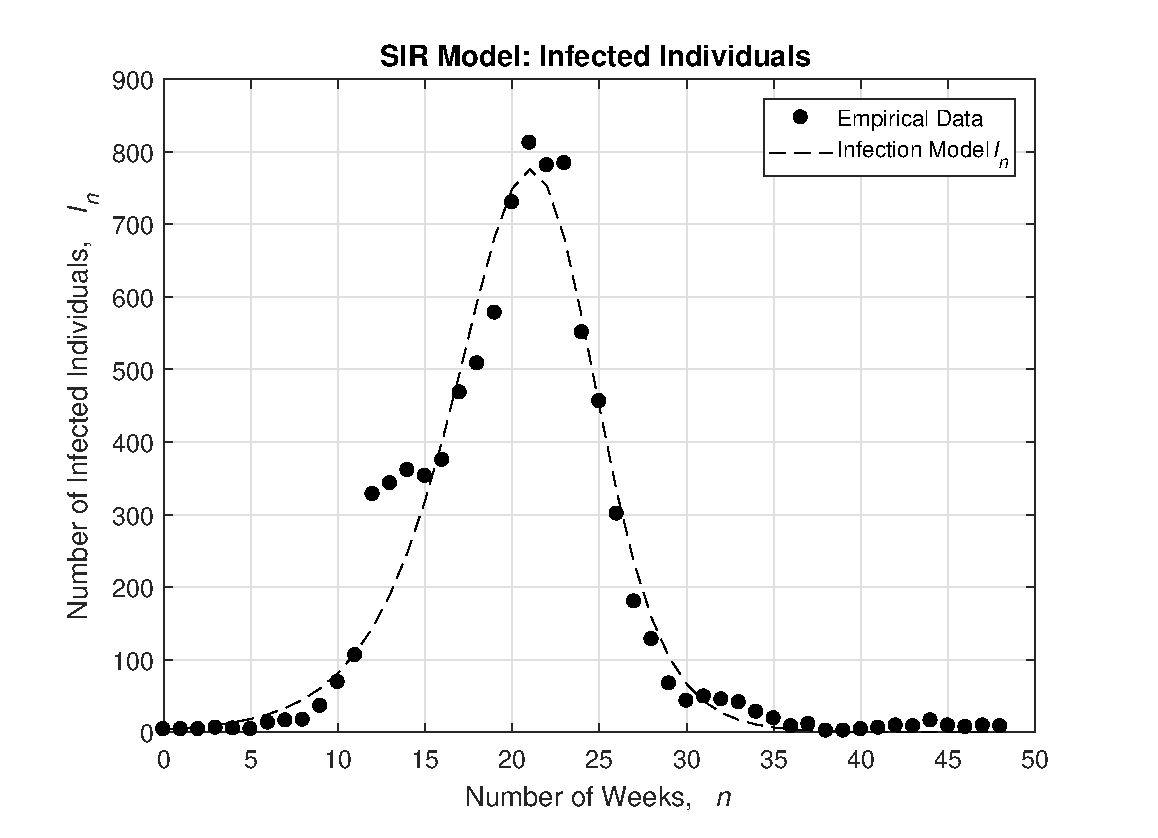
\includegraphics[width=15cm]{f1.eps}}
	\caption*{Figure 1}
\end{figure}





Figure 2 shows us the model for the number of susceptible people in the population. Those who have not contracted the flu are deemed susceptible, while those that have and those that have recovered are not considered susceptible. As one would expect, the greatest reduction in susceptible individuals is between 15 and 20 weeks, when infected cases are at their highest. For both Figure 1 and Figure 2, $\gamma$ was predicted to be 3.41, giving the average length of infectious period to be about 2 days. This gives a reasonable estimate of the infectious period of influenza and reflects many past doctors' advice to remain at home for at least 3 days when sick, accounting for slightly longer infectious periods.

\vspace{5mm}

\begin{figure}[H]
	\centering{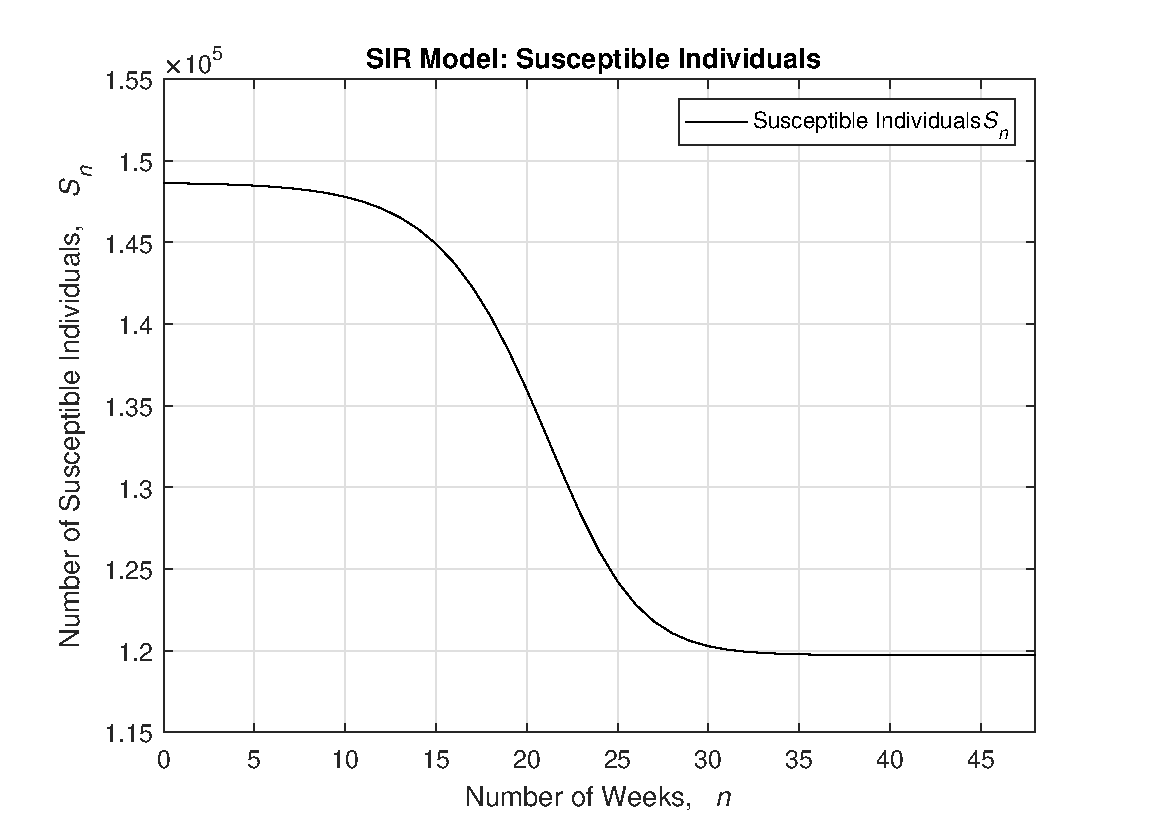
\includegraphics[width=15cm]{f2.eps}}
	\caption*{Figure 2}
\end{figure}

\vspace{5mm}



Figure 3 presents a comparison among the best fit data and 3 controls for spreading the flu: giving vaccinations to 6\% of the population, providing education on how to prevent the spread of disease, and using symptom shortening drugs like Tamiflu. These models are sown over 60 weeks. Clearly, the vaccine method is most effective. It is highly significant that just vaccinating 6\% of the population resulted in a 64\% decrease in total flu cases. This is a highly cost effective method for the consumer as flu vaccines can be found free or very cheaply. The cost associated with creating and distributing the vaccine is rather high, even when accounting for a world-wide market. The education control method is also highly effective, as more education about the spread of the virus will result in more effective self-quarantine. This is also cost effective, as adding such information to school curriculum, employee training videos, and public service announcements will not be a significant burden on the individual. The symptom drug method is clearly the least effective, with only an 18\% decrease in cases, and less cost effective as well. However, the drug model does predict a shorter outbreak period than the vaccine or education models, which still show some infected individuals after 50 weeks. 

\vspace{5mm}

\begin{figure}[H]
	\centering{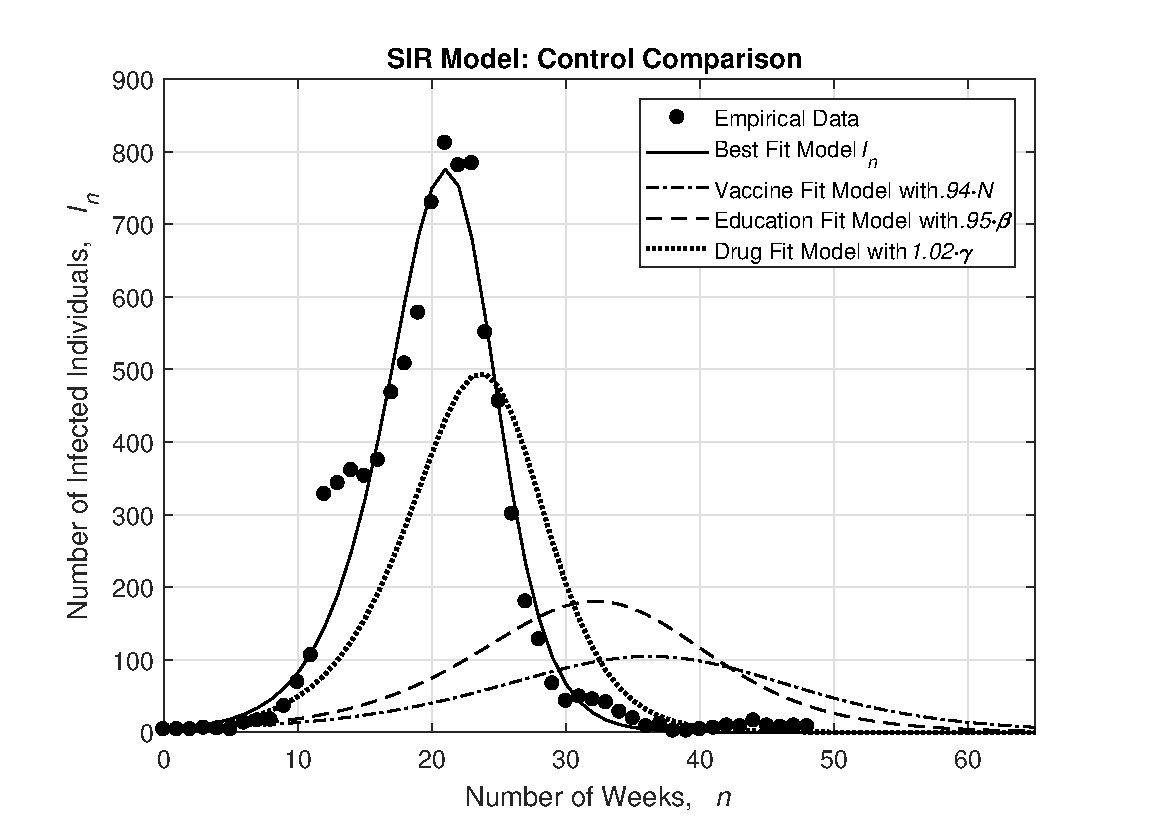
\includegraphics[width=15cm]{f3.eps}}
	\caption*{Figure 3}
\end{figure}

\vspace{5mm}



\section*{Equilibria and Linearizion}

We can find the equilibria of both the model for the infected population and the model for the susceptible population, which are interdependent. We will focus on non-negative values, as obtaining a negative value for a population model is not applicable. The model for the susceptible population is given by:

\vspace{5mm}

\begin{center}
	$S_{n+1}=S_n-\frac{\beta}{N}\cdot S_n\cdot I_n$
\end{center}

\vspace{5mm}

Setting $S_{n+1}=S_n$ we get:

\vspace{5mm}

\begin{center}
	$S_{n}=S_n-\frac{\beta}{N}\cdot S_n\cdot I_n \hspace{5mm} \longrightarrow \hspace{5mm} \frac{\beta}{N}\cdot S_n\cdot I_n=0$
\end{center}

\vspace{5mm}

So either $S_e=0$ or $I_e=0$. We can't analyze this model without a non-trivial value. Looking at the model for the infected population, we have:

\vspace{5mm}

\begin{center}
	$I_{n+1}=I_n+\frac{\beta}{N}\cdot S_n \cdot I_n-\gamma \cdot I_n$
\end{center}

\vspace{5mm}

Setting $I_{n+1}=I_n$ we have:

\vspace{5mm}

\begin{center}
	$I_{n}=I_n+\frac{\beta}{N}\cdot S_n \cdot I_n-\gamma \cdot I_n \hspace{5mm} \longrightarrow \hspace{5mm} I_n(\frac{\beta}{N}\cdot S_n-\gamma)=0$
\end{center}

\vspace{5mm}

So $I_e=0$ or $S_e=\gamma\cdot\frac{N}{\beta}$. We can now analyze the system with an equilibrium representative of zero infected individuals and some $S_e$ number of susceptible individuals. To linearize this system about the equilibria, first we must establish the matrix:

\vspace{5mm}

\begin{center}

\begin{Large}

$^{S_{n+1}}_{I_{n+1}}$\end{Large}$\hspace{3mm}=\hspace{3mm}$\begin{Large}$^{S_n-\frac{\beta}{N}\cdot S_n\cdot I_n}_{I_n(1+\frac{\beta}{N}\cdot S_n-\gamma)}$

\end{Large}

\end{center}

\vspace{5mm}

We can linearize this matrix by taking the partial derivatives of each expression for each variable ($I_n$ and $S_n$). We will consider both $S_{n+1}$ and $I_{n+1}$ to be functions of $S_n$ and $I_n$.

\vspace{5mm}

\begin{center}
	\begin{Large}

$^{\frac{\partial S_{n+1}}{\partial S_n} \hspace{5mm} \frac{\partial S_{n+1}}{\partial I_n}}_{\frac{\partial I_{n+1}}{\partial S_n} \hspace{5mm} \frac{\partial I_{n+1}}{\partial I_n}}$\end{Large}$\hspace{3mm}=\hspace{3mm}$\begin{Large}$^{1-\frac{\beta}{N}\cdot I_n \hspace{4mm} -\frac{\beta}{N}\cdot S_n}_{\frac{\beta}{N}\cdot I_n \hspace{10mm} 1+\frac{\beta}{N}\cdot S_n-\gamma}$

\end{Large}
\end{center}

\vspace{5mm}

We established that we want the equilibrium for $I_{n+1}$ to be zero. We will then say that the equilibrium   for $S_{n+1}$ is simply $S_e$. Plugging in the values of the equilibrium into out partial derivatives matrix, we get:

\vspace{5mm}

\begin{center}
	\begin{Large}

$^{1 \hspace{5mm} -\frac{\beta}{N}\cdot S_e}_{0 \hspace{5mm} 1+\frac{\beta}{N}\cdot S_e-\gamma}$

\end{Large}
\end{center}

\vspace{5mm} 

Taking the eigenvalues of this matrix tells us that for the equilibrium to be stable, $S_e$ must satisfy:

\vspace{5mm}

\begin{center}
	$ |\lambda_2|=|1+\frac{\beta}{N}\cdot S_e-\gamma| \leq 1 \hspace{5mm} \longrightarrow \hspace{5mm} 0\leq S_e \leq \gamma \cdot \frac{N}{\beta}$
\end{center}

\vspace{5mm}

Of course, there is the possibility that when these eigenvalues are equal to one the equilibrium is unstable or a saddle point, but for this analysis we will include one as a possibility. If we were to plug in our original optimized values for $N=148,632$, which were $\beta=3.7697$ and $\gamma=3.4128$, we would find that we obtain the inequality $0\leq S_e\leq 134,560$. This states that when the disease dies out (because we found $I_e=0$), our remaining population of susceptible individuals must be less than or equal to 135,560.  This is accurate, for we find that 119,720 is the equilibrium for $S_{n+1}$. 

Examining this inequality, we see that in order to decrease the total number of infected individuals (which would yield a higher number of susceptible individuals), we can take measures like decreasing the contact rate $\beta$ (through education and quarantine), or increasing the probability of recovery $\gamma$ (by using drugs like Tamiflu). Combining both of these measure will significantly decrease the total number of infected individuals, thus increasing our $S_e$. However, although vaccinations are very effective in controlling an outbreak, they do not influence the likelihood of the disease spreading and the threshold of the equilibrium in this case.

Another disease that satisfies this SIR model is the common cold. While we can't provide a vaccination for the hundreds of viral strains that are out there, we can provide education similar to influenza education to help reduce the total number of cases in an outbreak. Over-the-counter drugs for cold symptoms are readily available as well, and prescription antibiotics can often facilitate recovery quickly. In general, this study can provide insight into several other infectious diseases, particularly viral ones. The significant effectiveness of vaccines in relation to the small percentage of people who receive them is impressive. The current trend of "anti-vaxers" bodes ill for public health. We know that a small percentage of vaccinated individuals can make a huge difference, and conversely, when a small percentage {\it aren't} vaccinated the ramifications can be dangerous and wide-spread.



\section*{SIR Model with Birth and Death Factor}

Of course, there are far more complex SIR models that take several patterns into account. Considering birth and death rates would give our model a bit more complexity. Let us assume that the birth rate $b$ is equal to the death rate, which will keep our population constant. We can then model our susceptible $S$, our infected $I$, and our recovered $R$ for the influenza virus as:

\vspace{5mm}

$S_{n+1}=S_n-\frac{\beta}{N}\cdot S_n\cdot I_n+b(I_n+R_n)$

$I_{n+1}=I_n(1-\gamma-b)+\frac{\beta}{N}\cdot S_n \cdot I_n$

$R_{n+1}=R_n(1-b)+\gamma\cdot I_n$

\vspace{5mm}

Given these three equations, we know that our population $N$ is always equal to the sum of the susceptible, infected, and recovered (or, in this case, possibly $removed$). We can then use this relationship to model a difference equations for $S_n$ by setting $R_n=N-S_n-I_n$:

\vspace{5mm}

\begin{center}
	$S_{n+1}=S_n-\frac{\beta}{N}\cdot S_n\cdot I_n+b(N-S_n)$
\end{center}

\vspace{5mm}

And $I_{n+1}$ remains the same, as it does not explicitly include $R_n$. Unlike the previous section, we cannot assume that $I_e=0$. Finding the Equilibrium for $S_{n+1}=S_n$, we get:

\vspace{5mm}

\begin{center}
	{\large $S_e=\frac{b\cdot N}{I_n\cdot \frac{\beta}{N}+b}$}
\end{center}

\vspace{5mm}

And for $I_{n+1}=I_n$ we have

\vspace{5mm}

\begin{center}
	$I_e=0$ or $S_e=\frac{N}{\beta}\cdot (\gamma+b)$
\end{center}

\vspace{5mm}

This creates two sets of solutions for the SIR equilibrium model. If $I_{e1}=0$, then $S_{e1}=N$, which represents the population when no disease is present. Once influenza is introduced into the population, we can use substitution (and the fact that $R_0=\frac{\beta}{\gamma +b}$) to yield equilibria of $I_{e2}=b\cdot(R_0-1)\cdot \frac{N}{\beta}$ and $S_{e2}=\frac{N}{R_0}$. In order for these equilibria to be possible, we must have $R_0>1$. Otherwise, our values would not correspond to reality--our infected equilibria would be a negative number and our susceptible equilibria would be a number higher than the starting population.


Like in the previous section, we use the equilibria after linearizing the equations, then examine the eigenvalues. The Jacobian matrix is modeled as follows:

\vspace{5mm}

\begin{center}
	
	\begin{Large}
		
		$^{S_{n+1}}_{I_{n+1}}$\end{Large}$\hspace{3mm}=\hspace{3mm}$\begin{Large}$^{S_n-\frac{\beta}{N}\cdot S_n\cdot I_n+b(N-S_n)}_{I_n(1-\gamma-b)+\frac{\beta}{N}\cdot S_n \cdot I_n}\hspace{3mm}$
		
	\end{Large}
\end{center}

\vspace{5mm}

\begin{center}
	\begin{Large}
		
		$^{\frac{\partial S_{n+1}}{\partial S_n} \hspace{5mm} \frac{\partial S_{n+1}}{\partial I_n}}_{\frac{\partial I_{n+1}}{\partial S_n} \hspace{5mm} \frac{\partial I_{n+1}}{\partial I_n}}$\end{Large}$\hspace{3mm}=\hspace{3mm}$\begin{Large}$^{1-\frac{\beta}{N}\cdot I_n-b \hspace{4mm} -\frac{\beta}{N}\cdot S_n}_{\frac{\beta}{N}\cdot I_n \hspace{13mm} 1-\gamma-b+\frac{\beta}{N}\cdot S_n}$
		
	\end{Large}
\end{center}

\vspace{5mm}

And plugging in our equilibria  $I_{e1}$ and $S_{e1}$, we obtain:

\vspace{5mm}

\begin{center}
	\begin{Large}
		
		$^{1-b \hspace{5mm} -\beta}_{0 \hspace{9mm} 1-\gamma-b+\beta}$
		
	\end{Large}
\end{center}

\vspace{5mm}

This gives us eigenvalues $\lambda_{e1_1}=1-b$ and $\lambda_{e1_2}=1-\gamma-b+\beta$. In order to have a stable equilibria, we must have values that let both $\lambda_{e1_1}$ and $\lambda_{e1_2}$ be less than (or possibly equal to) 1. Again, even though stability at some $\lambda=1$ is not guaranteed, we will include it here. Since the birth/death rate for this constant population must always be $0\leq b < 1$, we know that $\lambda_{e1_1}$ fulfills the needed requirement for stability. Examining $\lambda_{e1_2}$, we can establish slightly stricter parameters:

\vspace{5mm}

\begin{center}
	$|1-\gamma-b+\beta|\leq1 \hspace{5mm} \longrightarrow \hspace{5mm} 0\leq\gamma+b+\beta\leq2 \hspace{5mm} \longrightarrow \hspace{5mm} -1\leq R_0\leq \frac{2}{\gamma+b}$
\end{center}

\vspace{5mm}

Since the reproduction number $R_0$ must be positive, we can just say that $R_0 \leq\frac{2}{\gamma+b}$ for a stable equilibria. Tiny values for $\gamma$ and $b$ will allow our value of $R_0$ to be very large and still produce a stable system. Conversely, for $\gamma$ and $b$ close to 1, our $R_0$ must be less than one in order to fulfill the requirements for a stable equilibria. In this situation, $\gamma$ and $b$ are generally small, which will ultimately result in $R_0$ greater than one.

Let's simulate the above model for $N=100$, $\beta=0.3$, $\gamma=0.2$, and $b=0.2$ with initial populations $S_0=70$ and $I_0=30$. Below shows a graph of this simulation over 25 weeks.

\begin{figure}[H]
	\centering{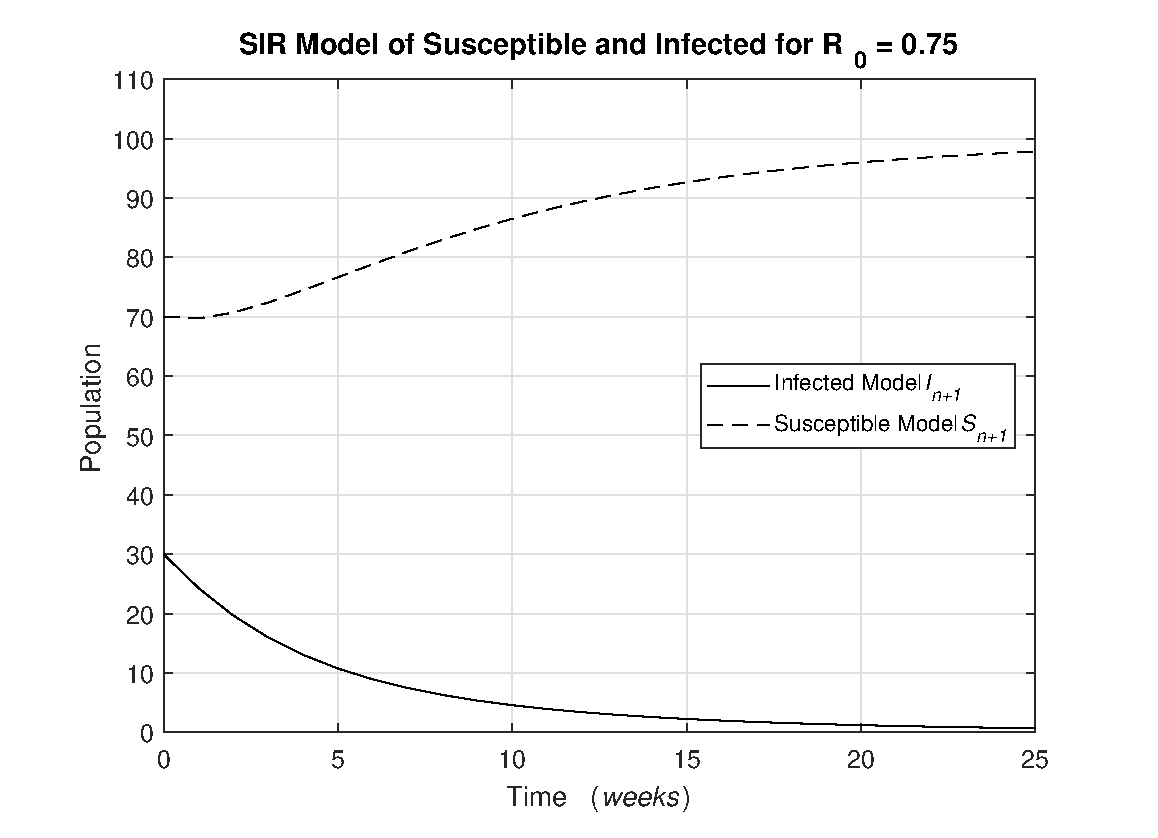
\includegraphics[width=14cm]{f4.eps}}
	\caption*{Figure 4}
\end{figure}

\vspace{5mm}

We can see that the number of infected individuals is headed towards an equilibrium of zero while the number of susceptible individuals is rising toward $N$. This correlates with our first set of equilibria found earlier. Here, $R_0=\frac{0.3}{0.2+0.2}=0.75<1$. If we were to examine other possible equilibria, we would obtain $I_e=-.25\cdot .2\cdot \frac{100}{0.3}\approx -17$ and $S_e=\frac{100}{.75}\approx 133$. These values do not make sense in reality, as we cannot have a negative value for the number of infected individuals nor a number larger than the population for the number of susceptible individuals.

To more closely examine the equilibria of the model above, we can linearize the equations. We will also examine all equilibria, even those less than zero. If we recall, our eigenvalues for the Jacobian matrix for $I_e=0$ and $S_e=N$ were given by  $\lambda_{e1_1}=1-b$ and $\lambda_{e1_2}=1-\gamma-b+\beta$. For this simulation, this corresponds to $\lambda_{e1_1}=.8$ and $\lambda_{e1_2}=.9$. Both have an absolute value less than one, so we can conclude that this equilibrium is stable.

Our other set of equilibrium values is for a population that is not disease-free. These correspond to $I_{e2}=b\cdot(R_0-1)\cdot\frac{N}{\beta}\approx-17 $ and $S_{e2}=\frac{N}{R_0}\approx 133$. Since $R_0<1$, these equilibria do not translate to a real-life population. However, we can still examine their stability. To evaluate the stability of these equilibria, we must also plug these into our Jacobian matrix and then find the eigenvalues. This yields:

\vspace{5mm}

\begin{center}
	{\Large $^{1-b\cdot R_0 \hspace{8mm} -\frac{\beta}{R_0}}_{b\cdot (R_0-1) \hspace{5mm} 1-\gamma-b+\frac{\beta}{R_0}} \hspace{5mm} \longrightarrow \hspace{5mm}	^{0.85 \hspace{6mm} -0.4}_{-0.5 \hspace{5mm} 1} \hspace{5mm} \longrightarrow \hspace{5mm} ^{1.3785 \hspace{4mm} 0}_{0 \hspace{11mm} .4715}$}
\end{center}

\vspace{5mm}

Giving us $\lambda_{e2_1}=1.3785$ and $\lambda_{e2_2}=.4715$. Since one of our eigenvalues is greater than one, this equilibrium is unstable.


We can simulate another model, this time with an $R_0$ greater than one. Here, we will keep the starting population at 100 but change $\beta=0.8$, $\gamma=0.1$, and $b=0.1$. The model below simulates these circumstances for 25 weeks.


We can see that with a higher $R_0$ of 4, we do not reach an equilibrium of 0. Our infected population is tending towards a rate of about 37\%. Here, the number of births and high contact rate ensure that there will always be a population of infected individuals, and the disease will not die out. 

\vspace{5mm}

\begin{figure}[H]
	\centering{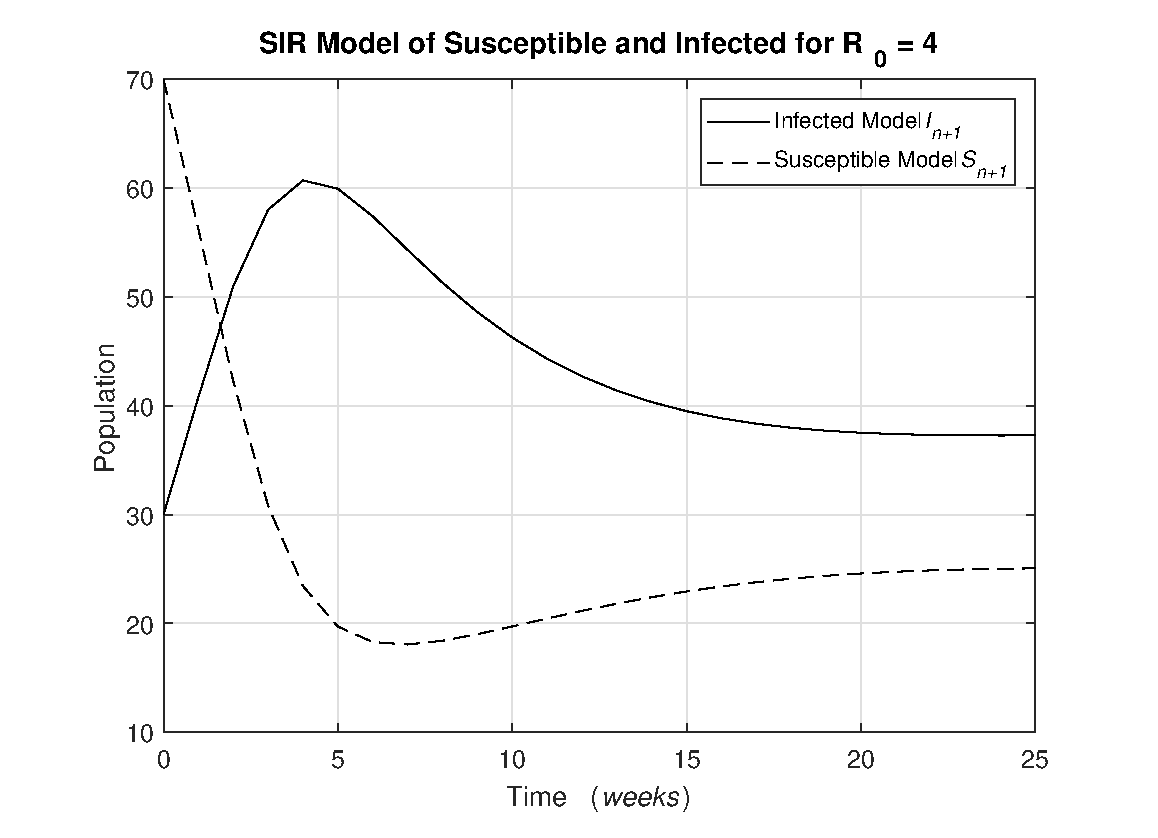
\includegraphics[width=14cm]{f5.eps}}
	\caption*{Figure 5}
\end{figure}

\vspace{5mm}


Let's examine the two sets of equilibria we found in the last section, $I_{e1}=0$ with $S_{e1}=N$, and $I_{e2}=b\cdot(R_0-1)\cdot \frac{N}{\beta}$ with $S_{e2}=\frac{N}{R_0}$. This corresponds to $I_{e1}=0$ with $S_{e1}=100$, and $I_{e2}=37.5$ with $S_{e2}=25$. Both sets of equilibria are plausible as actual population numbers, so we will see if they are stable or unstable. Let's use our previous eigenvalues of $\lambda_{e1_1}=1-b$ and $\lambda_{e1_2}=1-\gamma-b+\beta$, getting $\lambda_{e1_1}=.9$ and $\lambda_{e1_2}=1.6$. This tells us that the equilibrium is not stable, and the number of infected individuals cannot continue to be zero after even a small perturbation in the system. The model supports this, as the number of infected individuals does not tend towards zero.

For our second set of equilibria, we will need to revisit the Jacobian matrix and find our eigenvalues again. Doing this, we get:


\vspace{5mm}

\begin{center}
	{\Large $^{1-b\cdot R_0 \hspace{8mm} -\frac{\beta}{R_0}}_{b\cdot (R_0-1) \hspace{5mm} 1-\gamma-b+\frac{\beta}{R_0}} \hspace{5mm} \longrightarrow \hspace{5mm}	^{0.6 \hspace{5mm} -0.2}_{0.3 \hspace{5mm} 1} \hspace{5mm} \longrightarrow \hspace{5mm} ^{\frac{4}{5}+i\cdot \frac{\sqrt{2}}{10} \hspace{5mm} 0}_{0 \hspace{15mm} \frac{4}{5}-i\cdot \frac{\sqrt{2}}{10}}$}
\end{center}

\vspace{5mm}

Since we got complex numbers for our eigenvalues, we simply take the magnitude in order to determine the stability of the equilibria. Therefore, $|\lambda_{e2_1}|=.812404$ and $|\lambda_{e2_2}|=.812404$. Since both values are less than one, we can determine that this equilibrium is stable. Again, this is verified by the graph, as $S$ and $I$ tend toward constant values.

 
\end{document}





































